\documentclass[11pt,a4paper]{article}
\usepackage[utf8]{inputenc}
\usepackage[T1]{fontenc}
\usepackage[spanish,es-tabla,es-noshorthands]{babel}
\usepackage[a4paper,top=3.8cm,bottom=2.8cm,left=2cm,right=2cm,headheight=2.3cm,headsep=0.35cm,footskip=1.25cm]{geometry}
\usepackage[scaled=0.95]{helvet}
\renewcommand{\familydefault}{\sfdefault}
\usepackage{microtype}
\usepackage{array}
\usepackage{multirow}
\usepackage{tabularx}
\usepackage{longtable}
\usepackage{booktabs}
\usepackage{xcolor}
\usepackage{colortbl}
\usepackage{enumitem}
\usepackage{caption}
\usepackage{graphicx}
\usepackage{placeins}
\usepackage{lastpage}
\usepackage{fancyhdr}
\usepackage{eso-pic}
\usepackage{tikz}
\usepackage{tocloft}
\usepackage[hidelinks]{hyperref}

\newcolumntype{L}[1]{>{\raggedright\arraybackslash}p{#1}}
\newcolumntype{Y}{>{\raggedright\arraybackslash}X}
\captionsetup{font=small,labelfont=bf}
\setlist{itemsep=2pt,topsep=3pt}
\setlength{\parskip}{0.3em}
\setlength{\emergencystretch}{1.5em}

\definecolor{hdrgray}{gray}{0.85}

% indice: leaders punteados tambien en secciones
\renewcommand{\cftsecleader}{\cftdotfill{\cftdotsep}}
\renewcommand{\cftsecfont}{\bfseries}
\renewcommand{\cftsecpagefont}{\normalfont}
\setlength{\cftbeforesecskip}{4pt}

% caja de encabezado (cada pagina), a lo ancho del cuerpo
\newcommand{\encabezado}{\scriptsize
\setlength{\tabcolsep}{3pt}%
\begin{tabularx}{\textwidth}{|>{\centering\arraybackslash}m{4.6cm}|>{\centering\arraybackslash}X|>{\centering\arraybackslash}m{3.2cm}|}
\hline
\bfseries Pontificia Universidad Javeriana &
PROCESO\newline Ciclo de Desarrollo de Software\newline Documento: Proyecto - Entrega I &
Ingeniería en Sistemas\\
\hline
\end{tabularx}}

% caja de pie (cada pagina), a lo ancho del cuerpo
\newcommand{\piedepagina}{\scriptsize
\setlength{\tabcolsep}{3pt}%
\begin{tabularx}{\textwidth}{|m{4.6cm}|>{\centering\arraybackslash}X|>{\raggedleft\arraybackslash}m{3.2cm}|}
\hline
Joshua Mendez\newline Edinson Pedroza &
\begin{tabular}{@{}c@{}}Pontificia Universidad Javeriana\\ Ingeniería en Sistemas\end{tabular} &
Fecha: \today\newline Página \thepage{} de \pageref{LastPage}\\
\hline
\end{tabularx}}

\fancypagestyle{plantilla}{%
  \fancyhf{}%
  \renewcommand{\headrulewidth}{0pt}%
  \renewcommand{\footrulewidth}{0pt}%
  \fancyhead[C]{\encabezado}%
  \fancyfoot[C]{\piedepagina}%
}
% que el estilo "plain" (portada, índice) también use la plantilla
\fancypagestyle{plain}{%
  \fancyhf{}%
  \renewcommand{\headrulewidth}{0pt}%
  \renewcommand{\footrulewidth}{0pt}%
  \fancyhead[C]{\encabezado}%
  \fancyfoot[C]{\piedepagina}%
}

% borde de pagina alrededor del cuerpo
\AddToShipoutPictureBG{%
 \begin{tikzpicture}[remember picture,overlay]
  \draw[line width=0.5pt]
    ([xshift=2cm,yshift=2.35cm]current page.south west) rectangle
    ([xshift=-2cm,yshift=-3.6cm]current page.north east);
 \end{tikzpicture}}

\pagestyle{plantilla}

\begin{document}
\thispagestyle{plantilla}

% -------- PORTADA --------
\vspace*{5.5cm}
\begin{center}
{\fontsize{26}{30}\selectfont\bfseries PROYECTO DEL CURSO - ENTREGA I}\\[0.5cm]
{\large Sistema bajo prueba: Demoblaze}\\[1.6cm]
{\large\bfseries VERSIÓN 1.0}\\[2.5cm]
{\normalsize Joshua Mendez}\\[0.15cm]
{\normalsize Edinson Pedroza}\\[0.25cm]
{\normalsize Construcción de Software y Pruebas \quad Grupo A \quad 2026-2}\\[0.25cm]
{\normalsize Profesora: Claudia Martínez}
\end{center}
\clearpage

% -------- HOJA RESUMEN DE MODIFICACIONES --------
\phantomsection\addcontentsline{toc}{section}{Hoja resumen de modificaciones}
\vspace*{0.8cm}
\begin{center}\underline{\textbf{\large HOJA RESUMEN DE MODIFICACIONES}}\end{center}
\vspace{0.6cm}
{\small
\renewcommand{\arraystretch}{1.5}
\noindent\begin{tabularx}{\textwidth}{|c|c|Y|L{2.7cm}|L{2.7cm}|}
\hline
\rowcolor{black}
\textcolor{white}{\textbf{Versión}} & \textcolor{white}{\textbf{Fecha}} & \textcolor{white}{\textbf{Cambios respecto de la versión anterior}} & \textcolor{white}{\textbf{Preparado por}} & \textcolor{white}{\textbf{Aprobado por}}\\
\hline
1.0 & \today & Versión inicial & Joshua Mendez\newline Edinson Pedroza & Claudia Martínez\\
\hline
\end{tabularx}}
\clearpage

% -------- ÍNDICE --------
\renewcommand{\contentsname}{ÍNDICE}
\renewcommand{\cfttoctitlefont}{\hfill\large\bfseries}
\renewcommand{\cftaftertoctitle}{\hfill}
\tableofcontents
\clearpage

%==================================================================
%  SECCIONES 1 A 6
%==================================================================
%============================================================
%  ENTREGA I — SECCIONES 1 a 6 (cuerpo)
%  Requiere el preámbulo del plan: tabularx (col. L{} e Y),
%  booktabs, xcolor, hyperref, tikz, graphicx, enumitem.
%============================================================

%------------------------------------------------------------------
\FloatBarrier
\section*{1. Información general del proyecto}
\phantomsection\addcontentsline{toc}{section}{1. Información general del proyecto}

El sistema bajo prueba es \textbf{Demoblaze}, un sitio de terceros publicado por
BlazeMeter. El equipo no tiene su código fuente ni acceso al servidor, a la base de
datos o a los registros de aplicación: solo lo prueba por caja negra desde el
navegador. Por eso, las secciones que describen cómo está construido el sistema —en
especial la arquitectura— se basan en lo que se observa desde afuera (el tráfico HTTP
y los recursos que carga el navegador) y no en documentación interna del proveedor.

\begingroup
\small
\renewcommand{\arraystretch}{1.25}
\begin{table}[htb]\centering\small
\caption{Datos generales del proyecto y del sistema bajo prueba.}\label{tab:info-general}
\begin{tabularx}{\textwidth}{@{}L{4.4cm} Y@{}}
\toprule
\textbf{Elemento} & \textbf{Detalle} \\
\midrule
Nombre del software & Demoblaze \\
Tipo de sistema & Comercio electrónico: tienda en línea de demostración (\emph{demo e-commerce}). \\
URL de la aplicación & \url{https://www.demoblaze.com} \\
API que consume & \url{https://api.demoblaze.com} \\
Proveedor & BlazeMeter \\
Curso & Construcción de Software y Pruebas — Grupo A — 2026-2 \\
Profesora & Claudia Martínez \\
Institución & Pontificia Universidad Javeriana Cali \\
Entrega & Entrega I (100 pts) — fecha de entrega: 22 de octubre de 2026 \\
\bottomrule
\end{tabularx}
\end{table}
\endgroup

\subsection*{1.1 Integrantes del equipo}
\addcontentsline{toc}{subsection}{1.1 Integrantes del equipo}

\begingroup
\small
\renewcommand{\arraystretch}{1.25}
\begin{table}[htb]\centering\small
\caption{Integrantes del equipo.}\label{tab:integrantes}
\begin{tabularx}{\textwidth}{@{}L{6cm} Y@{}}
\toprule
\textbf{Integrante} & \textbf{Rol en la entrega} \\
\midrule
Joshua Mendez & Integrante \\
Edinson Pedroza & Integrante \\
\bottomrule
\end{tabularx}
\end{table}
\endgroup

\subsection*{1.2 Repositorio del código}
\addcontentsline{toc}{subsection}{1.2 Repositorio del código}

Aquí hay que hacer una distinción, porque el sistema bajo prueba no es del equipo.

\begin{itemize}
  \item \textbf{Código fuente de Demoblaze (el SUT): no disponible.} Demoblaze es un
        sitio de demostración de BlazeMeter, pensado para practicar automatización y
        QA. Su código fuente no es público y el equipo no tiene acceso al repositorio
        del proveedor, al servidor ni a la base de datos. Todo el trabajo se hace por
        caja negra desde el navegador. No se referencia ninguna URL de repositorio de
        Demoblaze porque no existe una pública que corresponda a este sistema.
  \item \textbf{Repositorio del equipo (artefactos de prueba): sí existe.} Lo que el
        equipo sí versiona es su propio trabajo: la suite de casos de prueba, el plan
        de pruebas, el registro de ejecución, los reportes de defectos y las
        evidencias. Ese es el repositorio que acompaña esta entrega.
\end{itemize}

\begingroup
\small
\renewcommand{\arraystretch}{1.25}
\begin{table}[htb]\centering\small
\caption{Repositorio de artefactos de prueba del equipo.}\label{tab:repo}
\begin{tabularx}{\textwidth}{@{}L{4.4cm} Y@{}}
\toprule
\textbf{Elemento} & \textbf{Valor} \\
\midrule
Repositorio del equipo (artefactos de prueba) & \url{https://github.com/JoshuaMontclair/demoblaze-pruebas-entrega1} \\
Contenido del repositorio & Suite de 68 casos de prueba (60 del plan + 8 de arreglos ortogonales), plan de pruebas, registro de ejecución, reportes de defectos y evidencias gráficas. \\
\bottomrule
\end{tabularx}
\end{table}
\endgroup

\noindent\emph{El repositorio contiene los artefactos de pruebas del equipo, no el código de Demoblaze (software de terceros).}

%------------------------------------------------------------------
\FloatBarrier
\section*{2. Descripción del sistema}
\phantomsection\addcontentsline{toc}{section}{2. Descripción del sistema}

\textbf{Qué es.} Demoblaze es una tienda en línea de demostración: reproduce el
comportamiento de un comercio electrónico real —catálogo de productos, detalle de
producto, carrito, registro, inicio de sesión y orden de compra— pero sin vender nada
de verdad ni cobrar pagos reales. Es un entorno de práctica estable y de acceso libre.

\textbf{Qué problema resuelve.} No resuelve un problema comercial; resuelve un problema
de formación y de herramientas. Quien aprende o ejercita pruebas de software necesita
un sistema realista contra el cual trabajar, que tenga flujos completos (navegar,
agregar al carrito, autenticarse, comprar) y que no imponga el riesgo de operar sobre
un sistema productivo real con datos o dinero de clientes. Demoblaze ofrece exactamente
eso: un e-commerce funcional, público y gratuito, que sirve de banco de pruebas para
diseñar casos, automatizar flujos y validar técnicas de testing.

\textbf{Quiénes lo usan.} Sus usuarios no son compradores reales, sino personas que
practican o enseñan calidad de software: estudiantes de pruebas, ingenieros de QA que
ensayan herramientas de automatización (Selenium, Playwright, Katalon y similares),
instructores que necesitan un sistema de ejemplo y equipos que evalúan frameworks de
prueba. Para el presente proyecto, el equipo lo usa como sistema bajo prueba de la
asignatura.

\textbf{Qué valor ofrece.} Un ambiente de práctica fiel a un comercio electrónico real,
disponible sin costo y sin necesidad de montar infraestructura propia. Al imitar los
módulos y las reglas de negocio de una tienda —el total es la suma de los ítems del
carrito, no se compra con el carrito vacío, el precio del listado coincide con el del
detalle— permite ejercitar pruebas funcionales, de integración de interfaz con
servicio, de seguridad básica y de rendimiento sobre un objetivo representativo. Que
sea un sistema de terceros, en producción y sin posibilidad de corregir sus defectos,
es parte de lo que lo hace un buen ejercicio: obliga a probar y documentar la calidad
observable desde afuera, que es la situación habitual cuando se audita un producto que
uno no construyó.

%------------------------------------------------------------------
\FloatBarrier
\section*{3. Arquitectura general}
\phantomsection\addcontentsline{toc}{section}{3. Arquitectura general}

La arquitectura que se describe aquí es la \textbf{inferida a partir de lo observable
desde el exterior}: el tráfico HTTP del navegador, los recursos que la página carga y
las respuestas del servicio. Al no tener acceso al código ni a la infraestructura del
proveedor, no se documenta la implementación interna (lenguaje del servidor, motor de
base de datos, despliegue), sino la forma en que el cliente y el servicio se comunican
tal como se ve desde el navegador.

\subsection*{3.1 Tecnologías observadas}
\addcontentsline{toc}{subsection}{3.1 Tecnologías observadas}

\begin{itemize}
  \item \textbf{Cliente web (frontend).} Es una aplicación de página única (SPA)
        servida como contenido estático desde \texttt{www.demoblaze.com}. Está
        construida con HTML, CSS y JavaScript, apoyada en \textbf{jQuery} para la
        manipulación del DOM y las llamadas al servicio, y en \textbf{Bootstrap} para
        la maquetación y los componentes visuales (grilla, modales, carrusel). La
        interfaz no calcula la lógica de negocio por su cuenta: delega en el servicio
        HTTP y pinta lo que este responde.
  \item \textbf{Servicio (backend).} Una \textbf{API HTTP de estilo REST} en
        \texttt{api.demoblaze.com} que responde en \textbf{JSON}. El frontend la
        consume para listar productos, filtrar por categoría, cargar el detalle de un
        producto, autenticar y operar el carrito y la orden. Entre las llamadas
        observadas en el tráfico están \texttt{GET /entries} (listado de productos),
        \texttt{POST /bycat} (productos por categoría), \texttt{POST /view} (detalle
        por identificador) y el servicio de \texttt{login}. Las operaciones de carrito
        y de compra también pasan por esta API.
  \item \textbf{Autenticación por token.} El inicio de sesión se resuelve contra el
        servicio: ante credenciales válidas, la API devuelve un \textbf{token de
        sesión} que el cliente usa para las operaciones que requieren usuario
        autenticado. (En el tráfico del login se observó, además, que la contraseña
        viaja codificada en base64 sobre HTTPS; esto es un hallazgo de seguridad
        documentado en el plan de pruebas, no una característica de diseño
        recomendable.)
  \item \textbf{Almacén de datos.} No es accesible ni inspeccionable, pero su
        existencia se infiere de que la API mantiene y devuelve de forma consistente
        los productos, categorías, usuarios registrados, el contenido del carrito y
        las órdenes. Se representa como un componente lógico ``almacén de datos''
        detrás de la API.
\end{itemize}

\subsection*{3.2 Componentes principales}
\addcontentsline{toc}{subsection}{3.2 Componentes principales}

\begin{enumerate}
  \item \textbf{Cliente web (SPA).} El navegador del usuario carga la página y sus
        recursos estáticos (HTML, JS, CSS, imágenes y el video de \emph{About us}) y
        ejecuta la lógica de presentación.
  \item \textbf{API REST.} Recibe las peticiones HTTP del cliente, devuelve JSON y
        concentra la lógica de negocio (catálogo, carrito, autenticación, compra).
  \item \textbf{Almacén de datos.} Guarda y provee la información que la API expone.
\end{enumerate}

La separación es nítida: el cliente es ``tonto'' respecto del negocio y el servicio es
quien decide. Esto quedó en evidencia durante las pruebas de integración, donde la
interfaz mostró \emph{undefined} al confiar en una respuesta \texttt{200 OK} que en
realidad traía \texttt{\{"errorMessage":"Not found."\}} para un producto inexistente
—es decir, el cliente pinta lo que el servicio le entrega sin validarlo por su cuenta.

\subsection*{3.3 Diagrama de arquitectura}
\addcontentsline{toc}{subsection}{3.3 Diagrama de arquitectura}

El flujo va de izquierda a derecha (Figura~\ref{fig:arquitectura}). Los componentes con
borde continuo (SPA, servidor estático y API) se \textbf{observan directamente} en el
tráfico del navegador; el almacén de datos va con borde punteado porque es un
componente \textbf{inferido}: no se inspecciona, pero su existencia se deduce de la
consistencia de las respuestas. El recuadro ``Infraestructura de BlazeMeter — caja
negra'' agrupa todo lo que es del proveedor y a lo que el equipo no tiene acceso.

\usetikzlibrary{arrows.meta,positioning,fit,backgrounds}
\begin{figure}[htb]\centering
\resizebox{\textwidth}{!}{%
\begin{tikzpicture}[
  font=\footnotesize,
  >={Latex[length=2.2mm]},
  box/.style   ={draw,rounded corners=2pt,align=center,inner sep=5pt,
                 fill=blue!6,line width=0.6pt,text width=2.9cm},
  store/.style ={draw,dashed,align=center,inner sep=5pt,
                 fill=violet!8,line width=0.9pt,text width=2.8cm},
  actor/.style ={draw,rounded corners=11pt,align=center,inner sep=6pt,
                 fill=gray!10,line width=0.6pt,text width=2.1cm},
  flow/.style  ={->,line width=0.7pt},
]
  \node[actor] (user) {Usuario\\\scriptsize(visitante o registrado)};
  \node[box, right=1.3cm of user]  (spa)      {SPA Demoblaze\\\scriptsize HTML/CSS/JS\\\scriptsize jQuery + Bootstrap};
  \node[box, right=3.1cm of spa]   (api)      {API REST\\\scriptsize\texttt{api.demoblaze.com}\\\scriptsize (respuestas JSON)};
  \node[box, above=0.95cm of api]  (estatico) {Servidor de contenido estático\\\scriptsize\texttt{www.demoblaze.com}};
  \node[store, right=1.5cm of api] (datos)    {Almacén de datos\\\scriptsize\textit{(inferido)}\\\scriptsize productos, usuarios, carritos y órdenes};

  \draw[flow] (user) -- node[above,font=\scriptsize]{interactúa} (spa);
  \draw[flow] (spa.north) |- node[above,pos=0.72,font=\scriptsize]{GET recursos estáticos} (estatico.west);
  \draw[flow] ([yshift=2.5mm]spa.east) -- node[above,align=center,font=\scriptsize]{HTTP + JSON\\/entries · /bycat · /view\\login · carrito · orden} ([yshift=2.5mm]api.west);
  \draw[flow] ([yshift=-2.5mm]api.west) -- node[below,font=\scriptsize]{token de sesión} ([yshift=-2.5mm]spa.east);
  \draw[flow] (api) -- node[above,align=center,font=\scriptsize]{consulta /\\actualiza} (datos);

  \begin{scope}[on background layer]
    \node[draw,dash pattern=on 3pt off 2pt,rounded corners,fill=gray!4,
          inner sep=11pt,fit=(estatico)(api)(datos),
          label={[font=\scriptsize\itshape]above:Infraestructura de BlazeMeter — caja negra}] {};
  \end{scope}
\end{tikzpicture}%
}
\caption{Arquitectura observada/inferida de Demoblaze. El cliente delega toda la lógica
de negocio en la API REST; el almacén de datos (borde punteado) es un componente
inferido a partir de la consistencia de las respuestas.}\label{fig:arquitectura}
\end{figure}

\subsection*{3.4 Descripción del diagrama (en prosa)}
\addcontentsline{toc}{subsection}{3.4 Descripción del diagrama (en prosa)}

El flujo va de izquierda a derecha. El \textbf{usuario} —sea visitante sin sesión o
usuario registrado— interactúa con la \textbf{SPA de Demoblaze} que se ejecuta en su
propio navegador. Esa aplicación de página única es HTML, CSS y JavaScript con jQuery y
Bootstrap, y se descarga como contenido estático desde \texttt{www.demoblaze.com}
(flecha de recursos estáticos hacia el \emph{servidor de contenido estático}).

Toda la lógica de negocio ocurre en el segundo salto: la SPA hace peticiones
\textbf{HTTP} a la \textbf{API REST} de \texttt{api.demoblaze.com}, que responde en
\textbf{JSON}. Por ese canal pasan el listado de productos (\texttt{/entries}), el
filtrado por categoría (\texttt{/bycat}), el detalle de producto (\texttt{/view}), el
inicio de sesión y las operaciones de carrito y de orden de compra. Cuando el usuario
se autentica correctamente, la API le devuelve a la SPA un \textbf{token de sesión},
que habilita las acciones propias del usuario registrado. Finalmente, la API consulta y
actualiza un \textbf{almacén de datos} que guarda productos, usuarios, carritos y
órdenes.

En el diagrama, los componentes con borde continuo (SPA, servidor estático y API) son
los que se \textbf{observan directamente} en el tráfico del navegador; el almacén de
datos va con borde punteado porque es un componente \textbf{inferido}: no se
inspecciona, pero su existencia se deduce de la consistencia de las respuestas. El
recuadro ``Infraestructura de BlazeMeter — caja negra'' agrupa todo lo que es del
proveedor y a lo que el equipo no tiene acceso.

%------------------------------------------------------------------
\FloatBarrier
\section*{4. Actores / tipos de usuario}
\phantomsection\addcontentsline{toc}{section}{4. Actores / tipos de usuario}

Demoblaze distingue, desde afuera, dos tipos de usuario según tengan o no una sesión
iniciada. No existe un panel de administrador accesible públicamente, así que no se
considera un tercer actor administrador.

\subsection*{4.1 Usuario visitante (sin sesión)}
\addcontentsline{toc}{subsection}{4.1 Usuario visitante (sin sesión)}

Es cualquier persona que entra al sitio sin autenticarse. Puede recorrer y operar casi
toda la tienda:

\begin{itemize}
  \item Ver el \textbf{catálogo} de productos en la página principal.
  \item Filtrar por las tres \textbf{categorías}: Phones, Laptops y Monitors.
  \item Navegar la \textbf{paginación} del listado.
  \item Abrir el \textbf{detalle} de un producto (nombre, precio, descripción e
        imagen).
  \item \textbf{Agregar productos al carrito} y ver el carrito, con el total como suma
        de los ítems, y la persistencia del contenido al navegar entre páginas.
  \item Eliminar productos del carrito.
  \item Abrir el formulario de \textbf{orden de compra} (Place Order), que presenta el
        total precargado y seis campos editables (Name, Country, City, Credit card,
        Month, Year).
  \item Enviar el formulario de \textbf{Contacto} (email, nombre, mensaje).
  \item \textbf{Registrarse} (Sign up) para crear una cuenta.
\end{itemize}

\subsection*{4.2 Usuario registrado (con sesión)}
\addcontentsline{toc}{subsection}{4.2 Usuario registrado (con sesión)}

Es el visitante que creó una cuenta (Sign up) y además inició sesión (Log in). La
sesión se sostiene mediante el token que devuelve la API. Además de todo lo que puede
hacer el visitante, el usuario registrado:

\begin{itemize}
  \item Opera el sitio con su \textbf{sesión identificada} (su nombre de usuario queda
        visible en la barra superior).
  \item Puede \textbf{cerrar sesión} (Log out).
  \item Completa el flujo de compra asociado a su cuenta.
\end{itemize}

\noindent\emph{Sobre la sesión y la compra (comportamiento real observado).} El sitio
permite abrir el formulario \emph{Place Order} y procede a validar sus campos antes que
la sesión: con el carrito vacío no deja completar la compra (regla R1), y en el
formulario, si faltan Name o Credit card, el sistema la rechaza con el mensaje
\texttt{Please fill out Name and Creditcard.} (regla R5). El comportamiento exacto
respecto de la sesión en el momento de confirmar la compra se documenta en el plan de
pruebas con su evidencia; aquí se describe el flujo tal como se observa desde la
interfaz.

\subsection*{4.3 Administrador}
\addcontentsline{toc}{subsection}{4.3 Administrador}

\textbf{No hay un actor administrador accesible públicamente.} Demoblaze no expone una
consola de administración ni funciones de gestión (altas de productos, gestión de
usuarios, reportes) a las que el equipo pueda llegar desde el navegador. Cualquier
administración del sitio es interna al proveedor (BlazeMeter) y queda fuera del alcance
observable, por lo que no se modela como actor del sistema bajo prueba.

%------------------------------------------------------------------
\FloatBarrier
\section*{5. Lista de funcionalidades del sistema}
\phantomsection\addcontentsline{toc}{section}{5. Lista de funcionalidades del sistema}

Una funcionalidad \textbf{con lógica de negocio} es aquella en la que el sistema aplica
un cálculo, una validación compuesta, un algoritmo de selección o una regla de
consistencia; no se limita a crear, leer, actualizar o borrar un registro. A
continuación se identifican cuatro funcionalidades de Demoblaze que cumplen ese
criterio.

\begingroup
\footnotesize
\setlength{\tabcolsep}{4pt}
\renewcommand{\arraystretch}{1.2}
\begin{table}[htb]\centering\footnotesize
\caption{Funcionalidades con lógica de negocio (no-CRUD).}\label{tab:funcionalidades}
\begin{tabularx}{\textwidth}{@{}c L{2.4cm} L{2.2cm} Y@{}}
\toprule
\textbf{\#} & \textbf{Funcionalidad} & \textbf{Actor} & \textbf{Descripción (lógica que la hace no-CRUD)} \\
\midrule
F1 & \textbf{Cálculo del total del carrito} & Cliente (comprador) &
El sistema no almacena un total fijo: lo \textbf{calcula} sumando el precio de cada
ítem presente en el carrito cada vez que se agrega o elimina un producto. El resultado
es una operación aritmética derivada del contenido actual del carrito, no un dato que
el usuario introduzca o edite. La prueba verifica que el total es igual a la suma de
los precios de los ítems ($\mathrm{TOTAL} = \sum$ precios) para uno y varios
productos (regla R3). \\
F2 & \textbf{Validación del flujo de compra (Place Order)} & Cliente (comprador, en sesión) &
El sitio decide si una compra procede combinando \textbf{tres condiciones}: que haya
una sesión iniciada, que el carrito no esté vacío y que los campos obligatorios estén
completos. Solo con las tres satisfechas se genera el comprobante; si falta cualquiera,
rechaza. Es una \textbf{validación compuesta} (modelada como tabla de decisión), no la
simple escritura de un formulario. Incorpora además la \textbf{precarga del total}
desde el carrito y las obligatoriedades de R1, R2 y R5. \\
F3 & \textbf{Filtrado del catálogo por categoría} & Visitante / Cliente &
Sobre el listado de productos, el sistema \textbf{selecciona y reconstruye} el conjunto
mostrado según la categoría elegida (Phones, Laptops, Monitors), pidiendo al servicio
solo los productos de esa clase y repintando la página. Es un \textbf{algoritmo de
filtrado} con un criterio de pertenencia, no la lectura plana de una lista completa. \\
F4 & \textbf{Consistencia de precio entre listado y detalle} & Visitante / Cliente &
El sistema expone el precio de un mismo producto en dos vistas (tarjeta del catálogo y
ficha de detalle) que se nutren del mismo servicio. La funcionalidad relevante es que
esos dos valores \textbf{deben coincidir}: es una \textbf{regla de consistencia de
datos} entre representaciones (regla R4), no un simple despliegue de información. \\
\bottomrule
\end{tabularx}
\end{table}
\endgroup

\subsection*{5.1 Funcionalidades excluidas por ser CRUD o acceso (no cuentan)}
\addcontentsline{toc}{subsection}{5.1 Funcionalidades excluidas por ser CRUD o acceso}

Las siguientes operaciones quedan \textbf{explícitamente fuera} de esta lista porque son
CRUD puro o control de acceso, sin lógica de negocio:

\begin{itemize}
  \item \textbf{Registro (Sign up):} alta de un usuario con usuario/contraseña. Es un
        \emph{create} de registro.
  \item \textbf{Autenticación (Log in / Log out):} validación de credenciales y
        apertura/cierre de sesión. Es control de acceso, no lógica de negocio del
        dominio.
  \item \textbf{Lectura del listado de productos y de la ficha de detalle} en sí mismas
        (el simple \emph{read}), separadas de las reglas de filtrado (F3) y de
        consistencia (F4) que sí aportan lógica.
\end{itemize}

\noindent\emph{Estas operaciones sí se prueban en la suite (módulos Registro y
Autenticación), pero como funcionalidades de tipo CRUD/acceso, no como funcionalidades
con lógica de negocio.}

%------------------------------------------------------------------
\FloatBarrier
\section*{6. Reglas de negocio identificadas}
\phantomsection\addcontentsline{toc}{section}{6. Reglas de negocio identificadas}

Reglas verificables desde afuera (caja negra), redactadas de forma formal. Cada una
indica qué implica para las pruebas. El criterio de referencia de R1–R6 son las
\textbf{convenciones del dominio} de comercio electrónico declaradas en el plan de
pruebas del equipo (apartado 3.4): ``que no deje comprar con el carrito vacío, que el
total dé igual a la suma de lo que muestra, que el precio del listado sea el mismo del
detalle y que un error de login no deje adivinar si el usuario existe''.

\begingroup
\footnotesize
\setlength{\tabcolsep}{4pt}
\renewcommand{\arraystretch}{1.2}
\begin{table}[htb]\centering\footnotesize
\caption{Reglas de negocio identificadas y su implicación para las pruebas.}\label{tab:reglas}
\begin{tabularx}{\textwidth}{@{}L{0.9cm} Y Y@{}}
\toprule
\textbf{Regla} & \textbf{Enunciado} & \textbf{Qué implica para las pruebas} \\
\midrule
\textbf{R1} & No se puede completar una compra con el \textbf{carrito vacío}: el sistema
debe rechazar el flujo de Place Order si no hay al menos un producto. &
Caso negativo con carrito vacío y campos completos (combinación de la tabla de
decisión): se verifica que no se genere comprobante. \\
\textbf{R2} & La compra se realiza \textbf{en el contexto de una sesión de usuario}:
aunque la ventana Place Order puede abrirse desde el carrito, el flujo de compra válido
(el que produce comprobante) está asociado a una sesión iniciada; sin sesión, el
sistema exige iniciarla. &
Casos que varían la condición ``sesión Sí/No'' manteniendo carrito y campos; se
documenta el comportamiento observado respecto a la sesión. \\
\textbf{R3} & El \textbf{total} mostrado en el carrito y en Place Order es igual a la
\textbf{suma de los precios} de los productos agregados; el total de Place Order viene
\textbf{precargado} desde el carrito y no es editable. &
Comparar el total con la suma calculada manualmente para 1 y N productos; verificar que
el total del comprobante coincide con el del carrito. \\
\textbf{R4} & El \textbf{precio en el listado} del catálogo es igual al \textbf{precio
en el detalle} del mismo producto. &
Revisión de consistencia: para una muestra de productos, cotejar precio de la tarjeta
contra precio de la ficha; cualquier diferencia es defecto. \\
\textbf{R5} & En Place Order, \textbf{Name y Credit card son obligatorios}; si faltan,
el sistema rechaza la compra con el mensaje exacto \texttt{Please fill out Name and
Creditcard.} &
Casos con Name y/o Credit card vacíos (y los demás campos completos): verificar el
mensaje exacto, que no se genere comprobante y que el carrito no se vacíe. \\
\textbf{R6} & El login con credenciales inválidas \textbf{no debe permitir la
enumeración de usuarios}: el mensaje para un usuario inexistente debe ser idéntico al
de una contraseña errada. &
Comparar la respuesta de usuario inexistente contra la de contraseña incorrecta; deben
ser indistinguibles. \emph{Observación:} los casos de seguridad del plan (CP-SEG-03 y
CP-SEG-05) confirmaron que Demoblaze \textbf{viola} esta regla, respondiendo
\texttt{User does not exist.} frente a \texttt{Wrong password.}, lo que sí permite
enumerar cuentas. \\
\textbf{R7} & El \textbf{contenido del carrito persiste} al navegar entre páginas
dentro de la misma sesión de navegación: los productos agregados no se pierden al
cambiar de vista. &
Agregar productos, navegar a otras páginas (catálogo, detalle) y regresar al carrito;
verificar que los ítems y el total se mantienen. \\
\bottomrule
\end{tabularx}
\end{table}
\endgroup

\subsection*{6.1 Nota de coherencia con el plan de pruebas}
\addcontentsline{toc}{subsection}{6.1 Nota de coherencia con el plan de pruebas}

R1, R3, R4 y R6 son exactamente las cuatro convenciones del dominio declaradas en el
apartado 3.4 del plan ya ejecutado. R2 y R5 formalizan las condiciones de la
\textbf{tabla de decisión de la compra} (apartado 3.3), donde el resultado esperado
depende de sesión, carrito y campos. R7 recoge la persistencia del carrito declarada en
el alcance del módulo Carrito. Las reglas de arriba sirven de criterio de referencia
(``resultado esperado'') para los casos de la suite de 60 pruebas del equipo.


%==================================================================
%  SECCIÓN 7 — DOCUMENTO DE PLAN DE PRUEBAS (resumen + remisión a Anexo A)
%==================================================================
\FloatBarrier
\section*{7. Documento de Plan de Pruebas}
\phantomsection\addcontentsline{toc}{section}{7. Documento de Plan de Pruebas}

El plan de pruebas y la estrategia de pruebas completos del proyecto —alcance, criterios
de entrada y salida (DoR/DoD), estrategia de pruebas, entregables, dependencias, entorno
de pruebas, gestión de riesgos y roles y responsabilidades— se desarrollan en el
documento de \textbf{Plan de Pruebas} del equipo, que se adjunta a esta entrega como
\textbf{Anexo A} (archivo \texttt{plan-completo-ejecutado.pdf}). Ese documento es, además,
la versión \emph{ejecutada} del plan: embebe los resultados reales de las pruebas de
integración, rendimiento, seguridad y compatibilidad con sus evidencias. Aquí se resumen
sus puntos clave y el detalle queda en el anexo.

\begin{itemize}
  \item \textbf{Alcance (sección 1 del plan).} Se prueba Demoblaze por caja negra sobre
        el entorno de producción del proveedor, cubriendo doce módulos (catálogo, detalle,
        carrito, registro, autenticación, orden de compra, contacto, interfaz y
        accesibilidad, rendimiento, integración sistema-producto, seguridad y
        compatibilidad). Quedan fuera las pruebas de componente e integración entre
        componentes (exigen el código fuente, no disponible) y las de denegación de
        servicio.
  \item \textbf{Criterios de entrada y salida (sección 2 del plan).} El DoR exige plan y
        casos aprobados, prueba de sanidad superada, navegador y datos de prueba
        definidos. El DoD fija dos criterios: \textbf{S1} —100\,\% de los casos de
        prioridad alta ejecutados y al menos el 80\,\% del total— y \textbf{S2} —al menos
        el 90\,\% de los casos ejecutados aprobados—, además del registro completo de
        defectos y el informe de resumen.
  \item \textbf{Estrategia de pruebas (sección 3 del plan).} Trabajo a nivel de sistema,
        con las cuatro técnicas de caja negra (partición de equivalencias, valores límite,
        tabla de decisión y arreglos ortogonales), priorización por riesgo (primero el
        flujo de compra), ejecución manual y criterios de referencia basados en estándares
        públicos: ISO/IEC 25010, WCAG 2.1, las métricas web esenciales de Google y las
        convenciones del dominio de comercio electrónico.
  \item \textbf{Entregables, dependencias y entorno (secciones 4 a 6 del plan).} Los
        entregables son el plan, la suite de casos, el registro de ejecución, el reporte
        de defectos, las evidencias y el informe de resumen. La dependencia principal es
        que el sitio —un servicio gratuito de un tercero, sin acuerdo de nivel de
        servicio— esté disponible; no hay un ambiente de pruebas separado, por lo que se
        prueba directamente sobre la producción compartida del proveedor.
  \item \textbf{Gestión de riesgos y roles (secciones 7 y 8 del plan).} Se usa una
        clasificación de severidad en tres niveles (crítico, medio, leve), se separan las
        restricciones asumidas (C1--C3) de los riesgos gestionables (R1--R6) y se asignan
        los roles de forma que el diseño de los casos (Joshua Mendez) y su ejecución
        (Edinson Pedroza) recaigan en personas distintas, para atenuar el sesgo de
        confirmación.
\end{itemize}

\noindent Para el detalle completo de cada punto, con sus tablas y evidencias, véase el
\textbf{Anexo A}.

%==================================================================
%  SECCIÓN 8 — DISEÑO Y DOCUMENTACIÓN DE CASOS (ARREGLOS ORTOGONALES)
%==================================================================
%==================================================================
% SECCIÓN 8 — Diseño y documentación de casos de prueba
% Entrega I · Construcción de Software y Pruebas · Grupo A · 2026-2
% Equipo: Joshua Mendez, Edinson Pedroza
% Cuerpo para \input dentro del documento maestro. Reutiliza la plantilla
% de plan-completo-ejecutado.tex: columnas L{} e Y, booktabs, tabularx a
% \textwidth y \footnotesize para las tablas anchas.
%==================================================================
\FloatBarrier
\section*{8. Diseño y documentación de casos de prueba}
\phantomsection\addcontentsline{toc}{section}{8. Diseño y documentación de casos de prueba}

\subsection*{8.1 Enfoque del diseño y técnicas de caja negra}
\addcontentsline{toc}{subsection}{8.1 Enfoque del diseño y técnicas de caja negra}

El diseño de casos para Demoblaze (\url{https://www.demoblaze.com}) se apoya en las
cuatro técnicas de diseño de caja negra que exige la rúbrica: \textbf{partición de
equivalencias}, \textbf{análisis de valores límite}, \textbf{tabla de decisión} y
\textbf{arreglos ortogonales}. Como el sistema es software de terceros —sin código
fuente ni acceso al servidor o a la base de datos—, todas las técnicas operan sobre
las entradas y salidas observables desde el navegador, que es justamente el ámbito de
la caja negra.

La suite completa está documentada en el anexo (hoja de cálculo con las columnas del
formato IEEE 829 y su registro de ejecución) y reúne \textbf{60 casos ya ejecutados},
cuyos resultados reales se consolidan en la sección 9. A esos 60 casos se suman
\textbf{8 casos nuevos de arreglos ortogonales} (\texttt{CP-AO-01} \dots{}
\texttt{CP-AO-08}), que completan la cuarta técnica y se desarrollan en el apartado
8.3. Con ello la suite alcanza \textbf{68 casos diseñados} en total.

\medskip
\noindent\textbf{Nota de integridad.} Los ocho casos \texttt{CP-AO} están
\emph{diseñados} en esta sección; su ejecución y resultados se reportan en la
sección 9. En este documento no se les atribuye ningún resultado de ejecución. Su
comportamiento esperado se deriva de las reglas de negocio observadas en el sistema y
está corroborado por los casos ya ejecutados \texttt{CP-COM-04}, \texttt{CP-COM-05} y
\texttt{CP-COM-06}, que ejercitan las mismas validaciones de obligatoriedad del
formulario de compra.

\subsection*{8.2 Cobertura por técnica de diseño}
\addcontentsline{toc}{subsection}{8.2 Cobertura por técnica de diseño}

La Tabla~\ref{tab:cobertura-tecnicas} resume cuántos casos aporta cada técnica. Las
cuatro técnicas de la rúbrica quedan cubiertas: las tres primeras ya ejecutadas dentro
de los 60 casos del plan, y los arreglos ortogonales mediante los 8 casos nuevos. Se
incluyen además la transición de estados (ciclo del carrito) y un bloque de técnicas
complementarias —comprobaciones de consistencia e inspección, más los casos de
integración, rendimiento, seguridad y compatibilidad— que no derivan de una técnica
formal de diseño de entradas pero forman parte de la suite ejecutada.

\begingroup
\small
\renewcommand{\arraystretch}{1.25}
\begin{table}[htb]\centering\small
\caption{Cobertura de la suite por técnica de diseño.}\label{tab:cobertura-tecnicas}
\begin{tabularx}{\textwidth}{@{}L{4.8cm} >{\centering\arraybackslash}p{1.5cm} L{3.4cm} Y@{}}
\toprule
\textbf{Técnica de diseño} & \textbf{N.\textsuperscript{o} de casos} & \textbf{Estado} & \textbf{Observación} \\
\midrule
Partición de equivalencias & 18 & Ejecutados (§9) & Campos de texto de los cuatro formularios (válido / inválido / vacío). \\
Valores límite & 2 & Ejecutados (§9) & Longitudes y bordes de mes/año del formulario de compra. \\
Tabla de decisión & 4 & Ejecutados (§9) & Combinaciones de sesión, carrito y campos de la compra. \\
\textbf{Arreglos ortogonales} & \textbf{8} & \textbf{Ejecutados (§9): 8/8 aprobados} & \textbf{Casos nuevos \texttt{CP-AO-01..08}; interacción por pares de los 6 campos de \emph{Place Order}.} \\
\midrule
Transición de estados & 11 & Ejecutados (§9) & Ciclo del carrito: vacío, con uno, con varios, tras eliminar y tras comprar. \\
Otras complementarias & 25 & Ejecutados (§9) & Consistencia, inspección, integración, rendimiento, seguridad y compatibilidad. \\
\midrule
\textbf{Total diseñado} & \textbf{68} & \multicolumn{2}{@{}l@{}}{\footnotesize 60 ejecutados (anexo, §9) + 8 arreglos ortogonales ejecutados (§9)} \\
\bottomrule
\end{tabularx}
\end{table}
\endgroup

Las cuatro técnicas de la rúbrica —partición de equivalencias, valores límite, tabla
de decisión y arreglos ortogonales— quedan así cubiertas. Las tres primeras ya
estaban ejercitadas en los 60 casos ejecutados; los arreglos ortogonales se añaden con
los ocho casos \texttt{CP-AO} que se diseñan a continuación.

\subsection*{8.3 Arreglos ortogonales (Taguchi): diseño de los casos CP-AO}
\addcontentsline{toc}{subsection}{8.3 Arreglos ortogonales (Taguchi): diseño de los casos CP-AO}

\subsubsection*{8.3.1 Por qué esta técnica y qué aporta a la suite}

La suite ya ejecutada aplica tres de las cuatro técnicas clásicas de caja negra. Falta
la cuarta, \textbf{arreglos ortogonales}, que es la que permite cubrir de forma
sistemática las \emph{combinaciones} entre varios parámetros de entrada. El arreglo
ortogonal resuelve un problema concreto: cuando un formulario tiene varios campos, el
número de combinaciones crece de forma exponencial y probarlas todas deja de ser
viable. Taguchi demostró que la mayoría de los defectos de interacción se disparan por
la combinación de \textbf{dos} factores a la vez, no por la de seis simultáneos. Un
arreglo ortogonal garantiza que \emph{todas las parejas} de niveles queden cubiertas
con una fracción mínima de corridas; esta propiedad se llama cobertura \textbf{pairwise}
(de a pares).

\subsubsection*{8.3.2 Función bajo prueba, factores y niveles}

Al pulsar \textbf{Place Order} sobre un carrito con productos, Demoblaze abre un
formulario con el total precargado y \textbf{seis campos editables}: Name, Country,
City, Credit card, Month y Year. Al pulsar \textbf{Purchase}, el sistema decide si
acepta o rechaza la compra en función de lo que tengan esos seis campos: una salida
que depende de la combinación de varios campos de entrada, que es el escenario para el
que sirve un arreglo ortogonal.

Tomamos los seis campos como \textbf{factores} y a cada uno le asignamos \textbf{dos
niveles} (rellenado-válido / vacío), que es la partición mínima y a la vez la más
informativa para una validación de obligatoriedad (regla R5). El dominio de valores
válidos ya se cubre con partición de equivalencias y valores límite en los casos
\texttt{CP-COM-05} y \texttt{CP-COM-06}; aquí no se repite ese trabajo, sino que se
estudia la \textbf{interacción entre los seis campos}.

\begingroup
\small
\renewcommand{\arraystretch}{1.2}
\begin{table}[htb]\centering\small
\caption{Factores y niveles del arreglo ortogonal.}\label{tab:factores}
\begin{tabularx}{\textwidth}{@{}>{\centering\arraybackslash}p{1.4cm} L{2.8cm} L{5.0cm} Y@{}}
\toprule
\textbf{Factor} & \textbf{Campo} & \textbf{Nivel 1 (rellenado-válido)} & \textbf{Nivel 2 (vacío)} \\
\midrule
A & Name & \texttt{Joshua Mendez} & \emph{(campo en blanco)} \\
B & Country & \texttt{Colombia} & \emph{(campo en blanco)} \\
C & City & \texttt{Bogotá} & \emph{(campo en blanco)} \\
D & Credit card & \texttt{4111\allowbreak1111\allowbreak1111\allowbreak1111} & \emph{(campo en blanco)} \\
E & Month & \texttt{12} & \emph{(campo en blanco)} \\
F & Year & \texttt{2030} & \emph{(campo en blanco)} \\
\bottomrule
\end{tabularx}
\end{table}
\endgroup

\subsubsection*{8.3.3 La explosión combinatoria: \texorpdfstring{$2^{6}=64$}{2\^{}6=64}}

Con 6 factores y 2 niveles cada uno, la combinación exhaustiva es

\[ 2^{6} = 2\times 2\times 2\times 2\times 2\times 2 = 64 \]

\noindent es decir, \textbf{64 corridas}. Para un solo formulario de una tienda de
demostración, probado a mano sobre un entorno de producción ajeno y compartido (véanse
las restricciones del plan de pruebas), 64 corridas son inviables y, sobre todo,
innecesarias: la enorme mayoría no aporta información nueva porque repite parejas de
condiciones ya vistas.

\subsubsection*{8.3.4 Arreglo ortogonal seleccionado: \texorpdfstring{L8 ($2^{7}$)}{L8 (2\^{}7)}}

Para 6 factores de 2 niveles, el arreglo de Taguchi más pequeño que los acomoda es el
\textbf{L8 ($2^{7}$)}: 8 corridas y hasta 7 columnas de 2 niveles. Usamos 6 de sus 7
columnas (una por factor) y dejamos la séptima sin asignar. El L8 reduce las 64
corridas exhaustivas a solo \textbf{8}. La Tabla~\ref{tab:l8-canonico} muestra la
matriz estándar en forma canónica y la Tabla~\ref{tab:l8-campos} la misma matriz
traducida a los valores de cada campo.

\begingroup
\small
\renewcommand{\arraystretch}{1.2}
\begin{table}[htb]\centering\small
\caption{Arreglo L8 en forma canónica. Cada fila es una corrida; el valor es el nivel (1 o 2) que toma el factor.}\label{tab:l8-canonico}
\setlength{\tabcolsep}{6pt}
\begin{tabular}{c cccccc c}
\toprule
\textbf{Corrida} & \textbf{A} & \textbf{B} & \textbf{C} & \textbf{D} & \textbf{E} & \textbf{F} & \textbf{Col.\,7} \\
 & {\scriptsize Name} & {\scriptsize Country} & {\scriptsize City} & {\scriptsize Card} & {\scriptsize Month} & {\scriptsize Year} & {\scriptsize (s/uso)} \\
\midrule
1 & 1 & 1 & 1 & 1 & 1 & 1 & 1 \\
2 & 1 & 1 & 1 & 2 & 2 & 2 & 2 \\
3 & 1 & 2 & 2 & 1 & 1 & 2 & 2 \\
4 & 1 & 2 & 2 & 2 & 2 & 1 & 1 \\
5 & 2 & 1 & 2 & 1 & 2 & 1 & 2 \\
6 & 2 & 1 & 2 & 2 & 1 & 2 & 1 \\
7 & 2 & 2 & 1 & 1 & 2 & 2 & 1 \\
8 & 2 & 2 & 1 & 2 & 1 & 1 & 2 \\
\bottomrule
\end{tabular}
\end{table}
\endgroup

\begingroup
\small
\renewcommand{\arraystretch}{1.2}
\begin{table}[htb]\centering\small
\caption{Arreglo L8 traducido a los campos. Nivel 1 = lleno, nivel 2 = vacío.}\label{tab:l8-campos}
\setlength{\tabcolsep}{5pt}
\begin{tabular}{c cccccc}
\toprule
\textbf{Corrida} & \textbf{Name} & \textbf{Country} & \textbf{City} & \textbf{Credit card} & \textbf{Month} & \textbf{Year} \\
\midrule
1 & lleno & lleno & lleno & lleno & lleno & lleno \\
2 & lleno & lleno & lleno & \textbf{vacío} & \textbf{vacío} & \textbf{vacío} \\
3 & lleno & \textbf{vacío} & \textbf{vacío} & lleno & lleno & \textbf{vacío} \\
4 & lleno & \textbf{vacío} & \textbf{vacío} & \textbf{vacío} & \textbf{vacío} & lleno \\
5 & \textbf{vacío} & lleno & \textbf{vacío} & lleno & \textbf{vacío} & lleno \\
6 & \textbf{vacío} & lleno & \textbf{vacío} & \textbf{vacío} & lleno & \textbf{vacío} \\
7 & \textbf{vacío} & \textbf{vacío} & lleno & lleno & \textbf{vacío} & \textbf{vacío} \\
8 & \textbf{vacío} & \textbf{vacío} & lleno & \textbf{vacío} & lleno & lleno \\
\bottomrule
\end{tabular}
\end{table}
\endgroup

\subsubsection*{8.3.5 Justificación de la reducción 64 \texorpdfstring{$\rightarrow$}{->} 8 y garantía pairwise}

¿Qué se pierde al pasar de 64 a 8 corridas? Nada de la cobertura de a pares, que es
donde se concentran los defectos de interacción. Un arreglo es \emph{ortogonal} cuando,
para \textbf{cualquier par de columnas}, las cuatro combinaciones posibles de sus
niveles —(1,1), (1,2), (2,1), (2,2)— aparecen \textbf{el mismo número de veces}. En el
L8 cada una aparece exactamente \textbf{dos veces} en cada par de columnas. Con 6
factores existen $C(6,2)=15$ parejas de campos, y el L8 cubre las cuatro combinaciones
de las 15 parejas en solo 8 corridas. La Tabla~\ref{tab:pairwise} lo verifica sobre la
pareja crítica Name--Credit card, que son los dos campos obligatorios según R5.

\begingroup
\small
\renewcommand{\arraystretch}{1.2}
\begin{table}[htb]\centering\small
\caption{Verificación de cobertura de la pareja crítica Name (A) -- Credit card (D).}\label{tab:pairwise}
\begin{tabularx}{\textwidth}{@{}L{5.4cm} Y >{\centering\arraybackslash}p{1.8cm}@{}}
\toprule
\textbf{Combinación (Name, Card)} & \textbf{Corridas donde aparece} & \textbf{Veces} \\
\midrule
(lleno, lleno) & 1, 3 & 2 \\
(lleno, vacío) & 2, 4 & 2 \\
(vacío, lleno) & 5, 7 & 2 \\
(vacío, vacío) & 6, 8 & 2 \\
\bottomrule
\end{tabularx}
\end{table}
\endgroup

Lo que el L8 \textbf{no} garantiza es la cobertura de interacciones de orden superior
(tres o más campos simultáneos en una combinación específica). Esa limitación es
aceptable y deliberada: la evidencia de Taguchi y de la literatura de \emph{pairwise
testing} indica que los fallos por combinación de tres o más factores son marginales
frente a los de a pares, y cubrirlos exigiría volver hacia las 64 corridas. Se cambia
un riesgo residual pequeño por una reducción del \textbf{87,5\,\%} en el número de
casos (de 64 a 8).

\textbf{¿Por qué 8 corridas y no 6?} Si el único objetivo fuera la cobertura pairwise
mínima, un \emph{covering array} lograría los 6 factores binarios en apenas 6 corridas.
Se usan 8 porque se exige la propiedad más fuerte de \textbf{arreglo ortogonal}: no
solo que cada par de niveles aparezca al menos una vez (covering array), sino que
aparezca el mismo número de veces (cobertura pairwise \emph{uniforme}, que obliga a que
el número de corridas sea múltiplo de 4). Esa uniformidad aporta balance estadístico
entre los factores —el fundamento del diseño de experimentos de Taguchi—; las 2
corridas extra son el precio de esa garantía de equilibrio.

\subsubsection*{8.3.6 Derivación del resultado esperado (R1, R3, R5)}

El resultado esperado de cada corrida no se inventa: se deduce de las reglas de negocio
observadas en el sistema.

\begin{itemize}
  \item \textbf{R1 — No se puede completar la compra con el carrito vacío.} Todas las
        corridas comparten la precondición de carrito con al menos un producto, de modo
        que R1 queda satisfecha y no es la variable bajo estudio. Por la misma razón, la
        \textbf{sesión iniciada} se fija como precondición constante y \textbf{no entra
        como factor}: el objetivo es la interacción entre los seis campos, no el efecto
        de la autenticación (que ya prueba por separado \texttt{CP-COM-03}).
  \item \textbf{R5 — Name y Credit card son obligatorios.} Si Name o Credit card quedan
        vacíos, el sistema rechaza la compra con el mensaje exacto ``Please fill out
        Name and Creditcard.'' y no genera comprobante. Esta es la regla que decide el
        resultado de cada corrida.
  \item \textbf{R3 — El total mostrado = suma de los precios de los productos.} Cuando
        la compra se completa, el monto del comprobante debe ser igual al total del
        carrito.
\end{itemize}

La regla operativa que se desprende de R5 es: la compra tiene éxito \emph{si, y solo
si}, Name y Credit card están ambos rellenados (con el carrito no vacío por R1). Los
campos Country, City, Month y Year no participan en la validación de obligatoriedad. La
Tabla~\ref{tab:derivacion} aplica esta regla a las 8 corridas.

\begingroup
\small
\renewcommand{\arraystretch}{1.2}
\begin{table}[htb]\centering\small
\caption{Derivación del resultado esperado de cada corrida (R1, R3, R5).}\label{tab:derivacion}
\begin{tabularx}{\textwidth}{@{}>{\centering\arraybackslash}p{1.3cm} >{\centering\arraybackslash}p{1.5cm} >{\centering\arraybackslash}p{1.7cm} >{\centering\arraybackslash}p{2.6cm} Y@{}}
\toprule
\textbf{Corrida} & \textbf{Name} & \textbf{Credit card} & \textbf{¿Ambos obligatorios llenos?} & \textbf{Resultado esperado} \\
\midrule
1 & lleno & lleno & Sí & Compra exitosa + comprobante (R3). \\
2 & lleno & vacío & No (falta tarjeta) & Rechazo: ``Please fill out Name and Creditcard.'' \\
3 & lleno & lleno & Sí & Compra exitosa + comprobante (R3). \\
4 & lleno & vacío & No (falta tarjeta) & Rechazo: ``Please fill out Name and Creditcard.'' \\
5 & vacío & lleno & No (falta nombre) & Rechazo: ``Please fill out Name and Creditcard.'' \\
6 & vacío & vacío & No (faltan ambos) & Rechazo: ``Please fill out Name and Creditcard.'' \\
7 & vacío & lleno & No (falta nombre) & Rechazo: ``Please fill out Name and Creditcard.'' \\
8 & vacío & vacío & No (faltan ambos) & Rechazo: ``Please fill out Name and Creditcard.'' \\
\bottomrule
\end{tabularx}
\end{table}
\endgroup

Resultado: \textbf{2 compras exitosas} (corridas 1 y 3) y \textbf{6 rechazos}
(corridas 2, 4, 5, 6, 7 y 8). La corrida \textbf{3} es la más interesante desde el
diseño: Name y Credit card están llenos, pero Country, City y Year quedan vacíos, y aun
así la compra se completa. Esto evidencia que, de los seis campos, el sistema solo
trata como obligatorios dos —el tipo de hallazgo que el arreglo ortogonal expone de
forma económica y que una sola prueba del ``camino feliz'' jamás mostraría—.

\subsubsection*{8.3.7 Casos de prueba formales (IEEE 829)}

Las 8 corridas se documentan como casos de prueba con el formato IEEE 829 de la suite
(ID, Módulo, Prioridad, Técnica de diseño, Precondiciones, Pasos, Datos de prueba,
Resultado esperado y Criterio de referencia). Los identificadores \texttt{CP-AO-01}
\dots{} \texttt{CP-AO-08} no colisionan con ningún ID de la suite. Para mantener la
tabla legible, las tres columnas que son idénticas en los ocho casos se declaran una
sola vez aquí, y la Tabla~\ref{tab:cp-ao} recoge las seis columnas restantes:

\begin{itemize}
  \item \textbf{Módulo:} Orden de compra.
  \item \textbf{Técnica de diseño:} Arreglos ortogonales.
  \item \textbf{Precondiciones:} sesión iniciada y carrito con al menos un producto;
        ventana \emph{Place Order} abierta.
\end{itemize}

\textbf{Criterio de priorización.} Las dos corridas de compra exitosa
(\texttt{CP-AO-01} y \texttt{CP-AO-03}) se marcan \textbf{Alta} porque ejercitan el
camino crítico del negocio —completar una compra—, prioridad máxima según el apartado
3.6 del plan. Las seis corridas de rechazo por R5 se marcan \textbf{Media}, en
coherencia con los casos negativos equivalentes de la suite (\texttt{CP-COM-05} y
\texttt{CP-COM-06}, también Media).

\medskip
\noindent\textbf{Estado de ejecución.} Los ocho casos de la Tabla~\ref{tab:cp-ao} están
\emph{diseñados} en esta sección; su ejecución y resultados se reportan en la
sección 9. No se consignan aquí resultados, capturas ni tiempos de ejecución. El
comportamiento esperado de los campos obligatorios ya está corroborado por los casos
ejecutados \texttt{CP-COM-04}, \texttt{CP-COM-05} y \texttt{CP-COM-06}.

\begingroup
\footnotesize
\setlength{\tabcolsep}{4pt}
\renewcommand{\arraystretch}{1.25}
\begin{longtable}{@{}L{1.5cm} L{1.0cm} L{3.1cm} L{2.8cm} L{3.4cm} L{2.8cm}@{}}
\caption{Casos de prueba de arreglos ortogonales en formato IEEE 829 (\texttt{CP-AO-01}--\texttt{CP-AO-08}). Módulo: Orden de compra; Técnica: Arreglos ortogonales; Precondiciones: sesión iniciada, carrito con al menos un producto y ventana \emph{Place Order} abierta.}\label{tab:cp-ao}\\
\toprule
\textbf{ID} & \textbf{Prior.} & \textbf{Pasos} & \textbf{Datos de prueba} & \textbf{Resultado esperado} & \textbf{Criterio de referencia} \\
\midrule
\endfirsthead
\multicolumn{6}{@{}l}{\footnotesize\emph{Tabla~\ref{tab:cp-ao} (continuación)}}\\
\toprule
\textbf{ID} & \textbf{Prior.} & \textbf{Pasos} & \textbf{Datos de prueba} & \textbf{Resultado esperado} & \textbf{Criterio de referencia} \\
\midrule
\endhead
\midrule
\multicolumn{6}{r@{}}{\footnotesize\emph{continúa en la página siguiente}}\\
\endfoot
\bottomrule
\endlastfoot
CP-AO-01 & Alta & 1.~Rellenar los seis campos con datos válidos. 2.~Pulsar Purchase. & Name: Joshua Mendez; Country: Colombia; City: Bogotá; Credit card: 4111\allowbreak1111\allowbreak1111\allowbreak1111; Month: 12; Year: 2030. & La compra se confirma y se muestra un comprobante con identificador, monto, titular y fecha. El monto es igual al total del carrito (R3). & Convención del dominio / R5: con Name y Credit card completados la compra procede; coherencia con R3 en el comprobante. \\
\midrule
CP-AO-02 & Media & 1.~Rellenar Name, Country y City. 2.~Dejar vacíos Credit card, Month y Year. 3.~Pulsar Purchase. & Name: Joshua Mendez; Country: Colombia; City: Bogotá; Credit card: (vacío); Month: (vacío); Year: (vacío). & El sistema rechaza la compra con el mensaje ``Please fill out Name and Creditcard.'' No genera comprobante ni vacía el carrito. & Convención del dominio / R5: Credit card es obligatorio. \\
\midrule
CP-AO-03 & Alta & 1.~Rellenar Name, Credit card y Month. 2.~Dejar vacíos Country, City y Year. 3.~Pulsar Purchase. & Name: Joshua Mendez; Country: (vacío); City: (vacío); Credit card: 4111\allowbreak1111\allowbreak1111\allowbreak1111; Month: 12; Year: (vacío). & La compra se confirma y se muestra el comprobante (monto = total del carrito, R3), aunque Country, City y Year estén vacíos. Evidencia que esos campos no son obligatorios. & Convención del dominio / R5: solo Name y Credit card son obligatorios; coherencia con R3. \\
\midrule
CP-AO-04 & Media & 1.~Rellenar Name y Year. 2.~Dejar vacíos Country, City, Credit card y Month. 3.~Pulsar Purchase. & Name: Joshua Mendez; Country: (vacío); City: (vacío); Credit card: (vacío); Month: (vacío); Year: 2030. & El sistema rechaza la compra con el mensaje ``Please fill out Name and Creditcard.'' No genera comprobante ni vacía el carrito. & Convención del dominio / R5: Credit card es obligatorio. \\
\midrule
CP-AO-05 & Media & 1.~Rellenar Country, Credit card y Year. 2.~Dejar vacíos Name, City y Month. 3.~Pulsar Purchase. & Name: (vacío); Country: Colombia; City: (vacío); Credit card: 4111\allowbreak1111\allowbreak1111\allowbreak1111; Month: (vacío); Year: 2030. & El sistema rechaza la compra con el mensaje ``Please fill out Name and Creditcard.'' No genera comprobante ni vacía el carrito. & Convención del dominio / R5: Name es obligatorio. \\
\midrule
CP-AO-06 & Media & 1.~Rellenar Country y Month. 2.~Dejar vacíos Name, City, Credit card y Year. 3.~Pulsar Purchase. & Name: (vacío); Country: Colombia; City: (vacío); Credit card: (vacío); Month: 12; Year: (vacío). & El sistema rechaza la compra con el mensaje ``Please fill out Name and Creditcard.'' No genera comprobante ni vacía el carrito. & Convención del dominio / R5: Name y Credit card son obligatorios. \\
\midrule
CP-AO-07 & Media & 1.~Rellenar City y Credit card. 2.~Dejar vacíos Name, Country, Month y Year. 3.~Pulsar Purchase. & Name: (vacío); Country: (vacío); City: Bogotá; Credit card: 4111\allowbreak1111\allowbreak1111\allowbreak1111; Month: (vacío); Year: (vacío). & El sistema rechaza la compra con el mensaje ``Please fill out Name and Creditcard.'' No genera comprobante ni vacía el carrito. & Convención del dominio / R5: Name es obligatorio. \\
\midrule
CP-AO-08 & Media & 1.~Rellenar City, Month y Year. 2.~Dejar vacíos Name, Country y Credit card. 3.~Pulsar Purchase. & Name: (vacío); Country: (vacío); City: Bogotá; Credit card: (vacío); Month: 12; Year: 2030. & El sistema rechaza la compra con el mensaje ``Please fill out Name and Creditcard.'' No genera comprobante ni vacía el carrito. & Convención del dominio / R5: Name y Credit card son obligatorios. \\
\end{longtable}
\endgroup

\subsubsection*{8.3.8 Resumen del bloque de arreglos ortogonales}

\begin{itemize}
  \item \textbf{Técnica:} arreglos ortogonales de Taguchi, la cuarta técnica de caja
        negra que completa la suite.
  \item \textbf{Factores:} los 6 campos de \emph{Place Order}, con 2 niveles cada uno
        (rellenado-válido / vacío).
  \item \textbf{Combinación exhaustiva:} $2^{6}=64$ corridas; \textbf{arreglo elegido:}
        L8 ($2^{7}$), que cubre todas las parejas de niveles (pairwise) en \textbf{8
        corridas}, una reducción del 87,5\,\%.
  \item \textbf{Resultados esperados:} derivados de R1, R3 y R5; 2 compras exitosas
        (\texttt{CP-AO-01}, \texttt{CP-AO-03}) y 6 rechazos con el mensaje ``Please fill
        out Name and Creditcard.''.
  \item \textbf{Hallazgo de diseño:} la corrida 3 muestra que de los 6 campos solo Name
        y Credit card son obligatorios.
  \item \textbf{Estado:} los ocho casos fueron \emph{ejecutados} (11-oct-2026) con
        resultado 8/8 aprobados; el detalle y las evidencias están en la sección 9.3.
\end{itemize}


%==================================================================
%  SECCIÓN 9 — REPORTE DE RESULTADOS Y EVIDENCIAS DE EJECUCIÓN
%==================================================================
\FloatBarrier
\section*{9. Reporte de resultados y evidencias de ejecución}
\phantomsection\addcontentsline{toc}{section}{9. Reporte de resultados y evidencias de ejecución}

Esta sección consolida los \textbf{resultados reales ya existentes} de la ejecución del
plan. El trabajo de ejecución se hizo sobre los \textbf{60 casos del plan} (identificadores
\texttt{CP-*}); su detalle caso por caso, con el registro de ejecución, el reporte de
defectos y las evidencias gráficas, está en el \textbf{Anexo A} (plan ejecutado) y en la
\textbf{suite de casos} (Anexo B, hojas \emph{Registro de ejecución} y \emph{Reporte de
defectos}). Las cifras de abajo se toman directamente de ese registro, sin redondeos que
favorezcan el resultado.

\subsection*{9.1 Resumen de ejecución}
\addcontentsline{toc}{subsection}{9.1 Resumen de ejecución}

\begingroup
\small
\renewcommand{\arraystretch}{1.3}
\begin{table}[htb]\centering\small
\caption{Resumen honesto de la ejecución (60 casos del plan).}\label{tab:resumen-ejec}
\begin{tabularx}{\textwidth}{@{}Y >{\raggedleft\arraybackslash}p{2.2cm} >{\raggedleft\arraybackslash}p{2.6cm}@{}}
\toprule
\textbf{Indicador} & \textbf{Casos} & \textbf{\% del registro} \\
\midrule
Casos del plan registrados          & 60 & 100,0\,\% \\
\midrule
\quad Aprobados                     & 24 & 40,0\,\% \\
\quad Fallidos                      & 20 & 33,3\,\% \\
\quad Bloqueados (restricción del plan) & 12 & 20,0\,\% \\
\quad No concluyentes               & 1  & 1,7\,\% \\
\quad No ejecutados (fin de ventana) & 3  & 5,0\,\% \\
\midrule
\textbf{Casos ejecutados (aprobados + fallidos)} & \textbf{44} & \textbf{73,3\,\%} \\
\bottomrule
\end{tabularx}
\end{table}
\endgroup

\begingroup
\small
\renewcommand{\arraystretch}{1.3}
\begin{table}[htb]\centering\small
\caption{Tasas derivadas y evaluación de los criterios de salida.}\label{tab:tasas}
\begin{tabularx}{\textwidth}{@{}L{6.6cm} >{\raggedright\arraybackslash}p{3.0cm} Y@{}}
\toprule
\textbf{Métrica / criterio} & \textbf{Valor} & \textbf{Estado} \\
\midrule
Cobertura de ejecución (44 ejecutados / 60 registrados) & 73,3\,\% & --- \\
Tasa de aprobación (24 aprobados / 44 ejecutados) & 54,5\,\% & --- \\
\midrule
S1. Cobertura de ejecución $\geq$ 80\,\% & 73,3\,\% & \textbf{No cumple} \\
S2. Tasa de aprobación $\geq$ 90\,\% & 54,5\,\% & \textbf{No cumple} \\
\bottomrule
\end{tabularx}
\end{table}
\endgroup

Ninguno de los dos criterios de salida se cumple, y conviene leer por qué sin maquillar
las cifras. La \textbf{tasa de aprobación} es del 54,5\,\% porque el sistema bajo prueba
es un sitio de demostración con defectos reales: los 20 casos fallidos no son errores de
ejecución, sino comportamientos defectuosos del producto que quedaron documentados (sección
9.2). Encontrar y registrar esos fallos es, de hecho, el objetivo del ejercicio sobre un
producto de terceros que no se puede corregir. La \textbf{cobertura} se queda en 73,3\,\%
por dos motivos trazables en el registro: 12 casos están \emph{bloqueados por las
restricciones del propio plan} —no se crean cuentas ni se escriben contraseñas en un sitio
ajeno (módulos Registro y Autenticación y el caso de compra con sesión), y las pruebas de
carga y estrés no se ejecutan sin un entorno propio ni autorización escrita del
propietario (restricción C1 del plan)—, y 4 casos más quedaron sin cerrar en la ventana de
trabajo (3 no ejecutados y 1 no concluyente). Si se descuentan los 12 casos no ejecutables
por restricción, la cobertura sobre lo que sí era ejecutable (44 de 48) sube al 91,7\,\%.

\subsection*{9.2 Defectos registrados}
\addcontentsline{toc}{subsection}{9.2 Defectos registrados}

La ejecución produjo \textbf{15 defectos}, clasificados por severidad según la sección 7
del plan. La Tabla~\ref{tab:def-sev} los resume por nivel y la Tabla~\ref{tab:def-lista}
los lista. El detalle completo (pasos de reproducción, resultado obtenido frente al
esperado y evidencia gráfica) está en el reporte de defectos de la suite (Anexo B) y en el
Anexo A.

\begingroup
\small
\renewcommand{\arraystretch}{1.3}
\begin{table}[htb]\centering\small
\caption{Defectos por severidad.}\label{tab:def-sev}
\begin{tabularx}{\textwidth}{@{}Y >{\raggedleft\arraybackslash}p{3cm}@{}}
\toprule
\textbf{Severidad} & \textbf{Cantidad} \\
\midrule
Crítico & 2 \\
Medio   & 9 \\
Leve    & 4 \\
\midrule
\textbf{Total} & \textbf{15} \\
\bottomrule
\end{tabularx}
\end{table}
\endgroup

\begingroup
\footnotesize
\setlength{\tabcolsep}{4pt}
\renewcommand{\arraystretch}{1.2}
\begin{longtable}{@{}L{1.3cm} L{1.4cm} L{3.0cm} L{10.3cm}@{}}
\caption{Listado de defectos registrados en la ejecución.}\label{tab:def-lista}\\
\toprule
\textbf{ID} & \textbf{Severidad} & \textbf{Módulo} & \textbf{Descripción} \\
\midrule
\endfirsthead
\multicolumn{4}{@{}l}{\footnotesize\emph{Tabla~\ref{tab:def-lista} (continuación)}}\\
\toprule
\textbf{ID} & \textbf{Severidad} & \textbf{Módulo} & \textbf{Descripción} \\
\midrule
\endhead
\midrule
\multicolumn{4}{r@{}}{\footnotesize\emph{continúa en la página siguiente}}\\
\endfoot
\bottomrule
\endlastfoot
DEF-03 & Crítico & Orden de compra & Se puede completar una compra con el carrito vacío y se emite un comprobante por 0 USD. \\
DEF-04 & Crítico & Orden de compra & El número de tarjeta no se valida: acepta letras y símbolos. \\
DEF-01 & Medio & Interfaz y accesibilidad & Las etiquetas de los formularios no están asociadas a sus campos (WCAG 1.3.1 y 4.1.2). \\
DEF-02 & Medio & Detalle de producto & Un producto inexistente se muestra como si existiera y se puede agregar al carrito. \\
DEF-05 & Medio & Orden de compra & La fecha del comprobante muestra el mes anterior al real. \\
DEF-06 & Medio & Contacto & El formulario de contacto acepta campos vacíos y correos con formato inválido. \\
DEF-07 & Medio & Rendimiento & Las métricas web esenciales no cumplen los umbrales, sobre todo en móvil. \\
DEF-10 & Medio & Seguridad & No se envía ninguna cabecera de seguridad HTTP. \\
DEF-12 & Medio & Seguridad & El login revela si un usuario existe (permite enumeración). \\
DEF-13 & Medio & Seguridad & La API acepta peticiones con credenciales desde cualquier origen (CORS mal configurado). \\
DEF-15 & Medio & Compatibilidad & En ancho de teléfono el menú no colapsa y el carrusel se ve vacío. \\
DEF-08 & Leve & Catálogo & El catálogo general y el filtro por categoría no son consistentes. \\
DEF-09 & Leve & Elementos de presentación & El video de About us se descarga en todas las páginas aunque nunca se muestre. \\
DEF-11 & Leve & Seguridad & La contraseña se envía en base64, que es reversible. \\
DEF-14 & Leve & Compatibilidad & En el motor de Firefox los enlaces del menú superior se parten en dos líneas. \\
\end{longtable}
\endgroup

Los dos defectos \textbf{críticos} están en el flujo de compra, que es el crítico del
negocio: se puede emitir un comprobante con el carrito vacío (DEF-03) y el número de
tarjeta no se valida (DEF-04). Entre los medios destacan los tres de seguridad confirmados
desde la API (DEF-10, DEF-12 y DEF-13) y el de accesibilidad de los formularios (DEF-01).

\subsection*{9.3 Ejecución de los casos de arreglos ortogonales (CP-AO)}
\addcontentsline{toc}{subsection}{9.3 Ejecución de los casos de arreglos ortogonales (CP-AO)}

Los \textbf{8 casos de arreglos ortogonales} (\texttt{CP-AO-01} \dots{} \texttt{CP-AO-08})
se \textbf{ejecutaron el 11 de octubre de 2026} sobre la versión en producción de Demoblaze
(\url{https://www.demoblaze.com}) en Google Chrome, usando el formulario \emph{Place Order}
con un carrito de un producto (Samsung galaxy s6, total 360 USD). Demoblaze emite sus
mensajes de validación mediante diálogos nativos de JavaScript (\texttt{alert}); para
ejecutar los casos de forma automatizada sin que esos diálogos bloquearan el navegador se
interceptó \texttt{window.alert} capturando su texto, \textbf{sin alterar la lógica de
validación} del sitio (técnica estándar de automatización de pruebas E2E).

\textbf{Resultado: los 8 casos se ejecutaron y los 8 pasaron} —el resultado real coincidió
con el esperado en todos—. No se encontraron defectos nuevos.

\begingroup
\footnotesize
\renewcommand{\arraystretch}{1.2}
\begin{table}[htb]\centering\footnotesize
\caption{Resultados reales de la ejecución de los casos de arreglos ortogonales.}\label{tab:cpao-ejec}
\begin{tabularx}{\textwidth}{@{}l L{4.4cm} Y c@{}}
\toprule
\textbf{Caso} & \textbf{Resultado esperado} & \textbf{Resultado real observado} & \textbf{Veredicto} \\
\midrule
CP-AO-01 & Compra exitosa + comprobante & Comprobante Id 4233245, Amount 360 USD, titular y tarjeta correctos & Pasó \\
CP-AO-02 & Rechazo (R5) & \texttt{"Please fill out Name and Creditcard."} & Pasó \\
CP-AO-03 & Compra exitosa + comprobante & Comprobante Id 6753988, Amount 360 USD, con Country/City/Year vacíos & Pasó \\
CP-AO-04 & Rechazo (R5) & \texttt{"Please fill out Name and Creditcard."} & Pasó \\
CP-AO-05 & Rechazo (R5) & \texttt{"Please fill out Name and Creditcard."} & Pasó \\
CP-AO-06 & Rechazo (R5) & \texttt{"Please fill out Name and Creditcard."} & Pasó \\
CP-AO-07 & Rechazo (R5) & \texttt{"Please fill out Name and Creditcard."} & Pasó \\
CP-AO-08 & Rechazo (R5) & \texttt{"Please fill out Name and Creditcard."} & Pasó \\
\midrule
\multicolumn{4}{@{}l@{}}{\footnotesize \textbf{8 ejecutados · 8 aprobados · 0 fallidos · 0 defectos nuevos} (tasa de aprobación 100\,\%).}\\
\bottomrule
\end{tabularx}
\end{table}
\endgroup

\textbf{Hallazgo confirmado.} El caso \texttt{CP-AO-03} completó la compra con Country, City
y Year vacíos, lo que \textbf{confirma empíricamente} que de los seis campos del formulario
solo \emph{Name} y \emph{Credit card} son obligatorios (regla R5). Además, en
\texttt{CP-AO-01} y \texttt{CP-AO-03} el monto del comprobante (360 USD) coincidió con el
total del carrito, confirmando también la regla R3. Estos ocho casos refuerzan lo ya
observado en los casos \texttt{CP-COM-04}, \texttt{CP-COM-05} y \texttt{CP-COM-06} del plan.

Las evidencias gráficas se encuentran en la carpeta \texttt{evidencias-cp-ao/}. Se muestran
dos a continuación:

\begin{figure}[htb]\centering
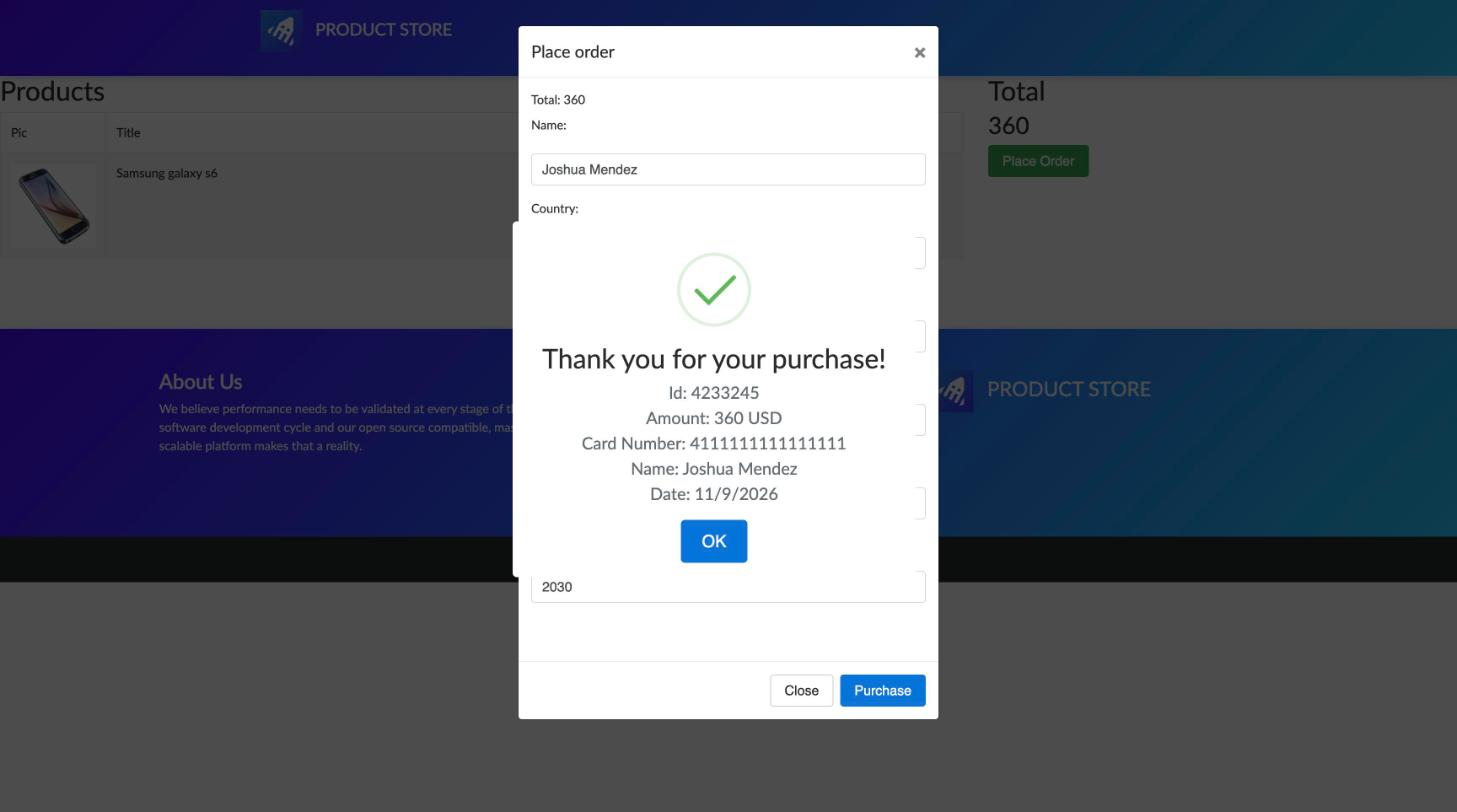
\includegraphics[width=0.78\textwidth]{evidencias-cp-ao/CP-AO-01_exito.jpg}
\caption{\texttt{CP-AO-01}: compra exitosa con los seis campos diligenciados (comprobante con monto igual al total del carrito).}
\end{figure}

\begin{figure}[htb]\centering
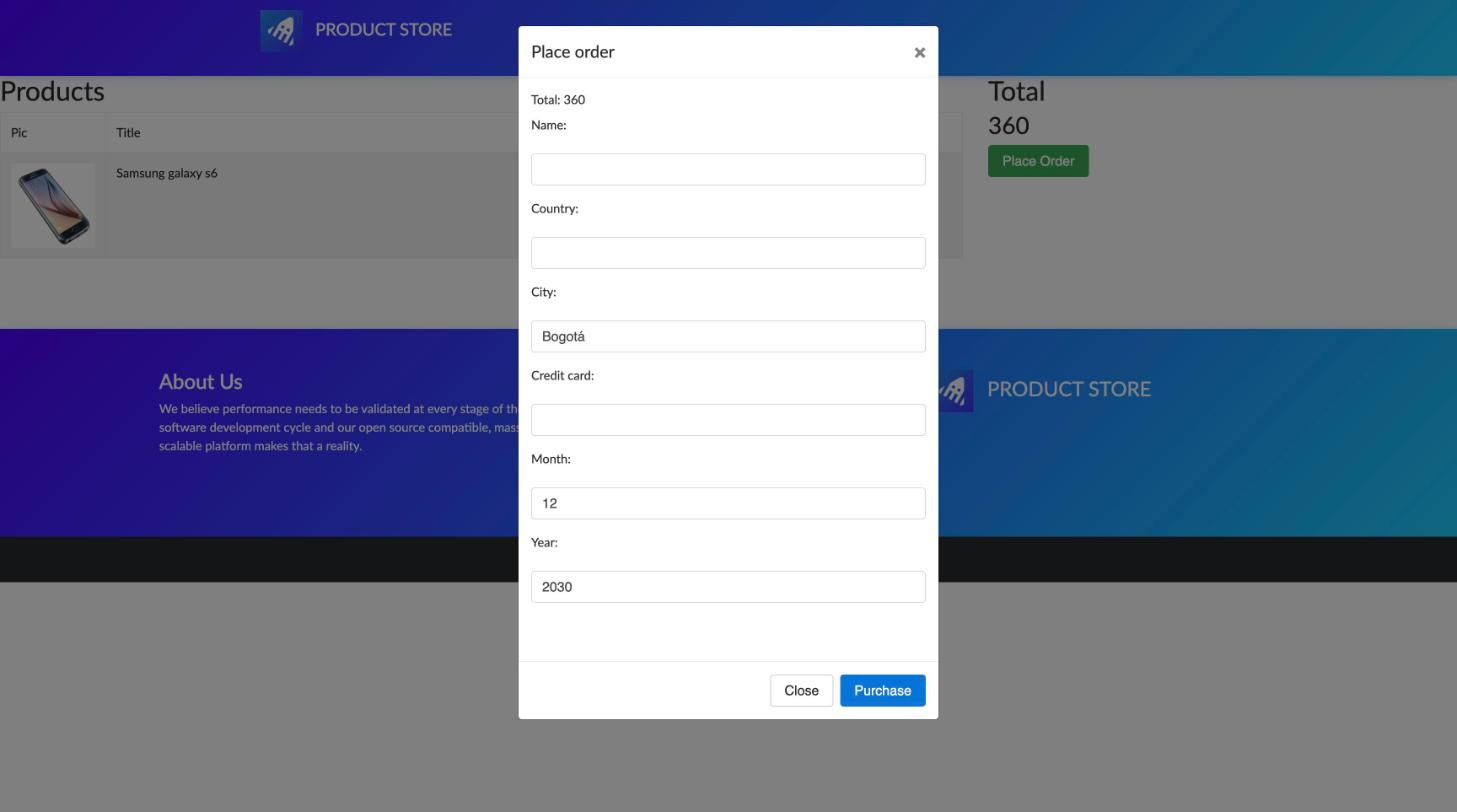
\includegraphics[width=0.78\textwidth]{evidencias-cp-ao/CP-AO-08_rechazo_form.jpg}
\caption{\texttt{CP-AO-08}: estado del formulario con \emph{Name}, \emph{Country} y \emph{Credit card} vacíos; al pulsar \emph{Purchase} el sistema rechazó la compra con el mensaje de validación.}
\end{figure}

%==================================================================
%  ANEXOS
%==================================================================
\FloatBarrier
\section*{Anexos}
\phantomsection\addcontentsline{toc}{section}{Anexos}

\subsection*{Anexo A — Plan de Pruebas (documento ejecutado)}
\addcontentsline{toc}{subsection}{Anexo A — Plan de Pruebas (documento ejecutado)}

Documento de plan de pruebas completo y ejecutado del proyecto, en PDF:
\texttt{plan-\allowbreak{}completo-\allowbreak{}ejecutado.pdf}. Contiene el desarrollo íntegro del plan (alcance,
DoR/DoD, estrategia, entregables, dependencias, entorno, gestión de riesgos y roles) y el
reporte de ejecución con evidencias gráficas de las pruebas de integración, rendimiento,
seguridad y compatibilidad. Es la fuente de las cifras consolidadas en la sección 9 de este
documento.

\subsection*{Anexo B — Suite de casos de prueba}
\addcontentsline{toc}{subsection}{Anexo B — Suite de casos de prueba}

Hoja de cálculo \texttt{suite-casos-de-prueba-entrega1.xlsx}, con cuatro hojas:

\begin{itemize}
  \item \textbf{Casos de prueba:} los 68 casos diseñados (60 del plan + 8 arreglos
        ortogonales \texttt{CP-AO}), con las columnas del formato IEEE 829 (ID, módulo,
        prioridad, técnica de diseño, precondiciones, pasos, datos de prueba, resultado
        esperado y criterio de referencia).
  \item \textbf{Registro de ejecución:} el resultado real de cada caso ejecutado del plan,
        con fecha, versión del navegador, resultado y referencia a la evidencia. Los ocho
        \texttt{CP-AO} se ejecutaron el 11 de octubre de 2026 (8 aprobados, 0 fallidos);
        su resultado se detalla en la sección 9.3 y sus evidencias en \texttt{evidencias-cp-ao/}.
  \item \textbf{Reporte de defectos:} los 15 defectos registrados, con pasos de
        reproducción, resultado obtenido frente al esperado, severidad y evidencia.
  \item \textbf{Resumen:} métricas de diseño, ejecución y defectos calculadas con fórmulas
        sobre las demás hojas.
\end{itemize}

\end{document}
